\chapter{Introduction}
\label{ch:introduction}

\section{Clinical Background and Epidemiological Context}
Breast cancer represents one of the most formidable global health challenges of the modern era, ranking as the most commonly diagnosed malignancy and a leading contributor to cancer-related mortality among women worldwide \citep{Sung2021}. According to the World Health Organization (WHO) and GLOBOCAN statistics, female breast cancer accounts for approximately 2.3 million new diagnoses annually, representing nearly 11.7\% of all global cancer cases \citep{Sung2021}. In oncological practice, clinical prognosis and long-term overall survival rates correlate directly with early detection: identifying neoplastic lesions at stage 0 (carcinoma in situ) or stage I yields a 5-year relative survival rate exceeding 99\%, whereas diagnosis at stage IV drops 5-year survival precipitously below 30\% \citep{Shen2019}.

To achieve early intervention, healthcare infrastructures rely upon systematic radiological screening modalities. Full-Field Digital Mammography (FFDM) serves as the primary population-wide screening standard; however, mammographic sensitivity degrades significantly in patients presenting with dense fibroglandular breast parenchyma (American College of Radiology BI-RADS density categories C and D) \citep{Shen2019, Mendelson2013}. In dense tissue, high-attenuation fibroglandular tissue visually overlaps and occludes microcalcifications and small solid tumors, causing mammographic sensitivity to plummet from over 85\% in fatty breasts down to under 50\% in extremely dense breasts \citep{Mendelson2013}. 

Medical Breast Ultrasound (BUS) has emerged as an indispensable complementary diagnostic imaging modality, serving as the frontline screening tool for younger cohorts, pregnant patients, and women with dense breast tissue \citep{AlDhabyani2020}. Operating without ionizing radiation, breast sonography utilizes high-frequency acoustic waves (typically 7 to 15 MHz) to achieve real-time, high-contrast visualization of soft-tissue interfaces \citep{Sikhakhane2024}. It provides vital diagnostic differentiation between benign fluid-filled simple cysts and solid neoplastic masses, whilst enabling real-time ultrasound-guided needle biopsies \citep{Stavros1995}.

\section{Challenges in Clinical Ultrasonography}
Despite its extensive diagnostic utility, the clinical efficacy of breast ultrasound is intrinsically constrained by two major operational vulnerabilities:

\begin{enumerate}
    \item \textbf{Acoustic Speckle Noise and Low Contrast:} Due to the physical wave mechanics of ultrasound propagation through heterogeneous biological parenchyma, sonograms are heavily corrupted by multiplicative acoustic speckle noise \citep{Sikhakhane2024}. The superposition of backscattered acoustic waves from cellular microstructures produces granular, signal-dependent intensity fluctuations that blur delicate lesion boundaries, mask subtle acoustic shadowing, and reduce the effective Contrast-to-Noise Ratio (CNR) \citep{Jiang2023}.
    \item \textbf{Inter-Observer Variability and Cognitive Fatigue:} Sonographic examination is operator-dependent and involves subjective real-time visual interpretation. Studies indicate inter-radiologist disagreement rates of up to 30\% when evaluating subtle morphological margin characteristics (such as microlobulation or angular margins) \citep{Litjens2017}. High clinical workloads and cognitive fatigue exacerbate the risk of false positives (triggering unnecessary benign tissue biopsies and patient anxiety) and false negatives (delaying critical therapeutic intervention) \citep{Kelly2019}.
\end{enumerate}

To overcome these diagnostic bottlenecks and establish a standardized clinical baseline, the biomedical imaging community has focused on Computer-Aided Diagnosis (CAD) systems powered by artificial intelligence \citep{Cheng2016}.

\section{Emergence of Deep Learning in Sonography}
Early CAD architectures deployed in the 1990s and 2000s relied on hand-engineered mathematical feature extractors, such as Gray-Level Co-occurrence Matrices (GLCM), Gabor texture filter banks, and boundary-tracking active contour models paired with classical classifiers such as Support Vector Machines (SVMs) \citep{Cheng2016}. While foundational, these classical systems exhibited acute brittleness, frequently generating high false-positive rates when confronted with varying scanner gain settings and acoustic shadowing artifacts \citep{Drukker2002}.

The advent of Deep Convolutional Neural Networks (CNNs) has fundamentally reshaped medical image computing \citep{Litjens2017}. Rather than relying on human-engineered heuristic descriptors, deep neural networks autonomously learn hierarchical spatial representations directly from raw acoustic pixel matrices \citep{He2016}. Early convolutional kernels detect fundamental low-level primitives (such as acoustic edges, gradients, and echogenic boundaries), while deeper residual blocks synthesize complex high-level diagnostic representations corresponding to clinical BI-RADS descriptors (including posterior acoustic attenuation, boundary spiculation, and hypoechoic tissue invasion) \citep{He2016, Mendelson2013}. 

Through transfer learning on massive visual repositories (such as ImageNet), deep CNN backbones (e.g., ResNet-50 and EfficientNet-B0) can generalize effectively across biomedical domains, overcoming the clinical scarcity of large-scale annotated ultrasound training sets \citep{Tan2019, AlDhabyani2020}.

\section{Problem Statement and Theoretical Motivation}
Despite remarkable empirical achievements on curated public benchmarks, the translation of deep learning ultrasound classifiers into uncurated clinical environments remains obstructed by two fundamental technical failures:

\begin{enumerate}
    \item \textbf{Vulnerability to Out-of-Distribution Acoustic Noise:} Deep learning models are mathematically optimized under the assumption that training and deployment data are drawn from identical underlying statistical distributions. When models trained on pristine or heavily filtered scans encounter real-world acoustic noise, standard pooling layers (e.g., Max Pooling) propagate peak noise spikes through hidden activations \citep{Jiang2023}. This corrupts the latent feature manifold, leading to catastrophic prediction errors and severe overconfidence on corrupted inputs.
    \item \textbf{Geometric Aspect Ratio Distortion in Standard Preprocessing:} Modern convolutional backbones require fixed square input tensors (typically $224 \times 224 \times 3$). Standard deep learning data loaders routinely apply direct anamorphic resizing to rectangular raw scans ($700 \times 500$ pixels). This non-uniform spatial scaling squishes the image, introducing an average geometric distortion error of $\mathcal{AR} = +38.5\%$. In clinical oncology, the ratio of lesion height to width ($H/W$) is a cardinal BI-RADS biomarker: malignant masses grow vertically across anatomical tissue planes yielding "taller-than-wide" shapes ($H/W > 1.0$), whereas benign fibroadenomas orient horizontally ($H/W < 1.0$) \citep{Stavros1995, Mendelson2013}. Direct anamorphic resizing artificially flattens taller-than-wide malignant tumors into squished, oval profiles, misleading convolutional spatial feature extractors and degrading diagnostic accuracy.
\end{enumerate}

\begin{figure}[htbp]
    \centering
    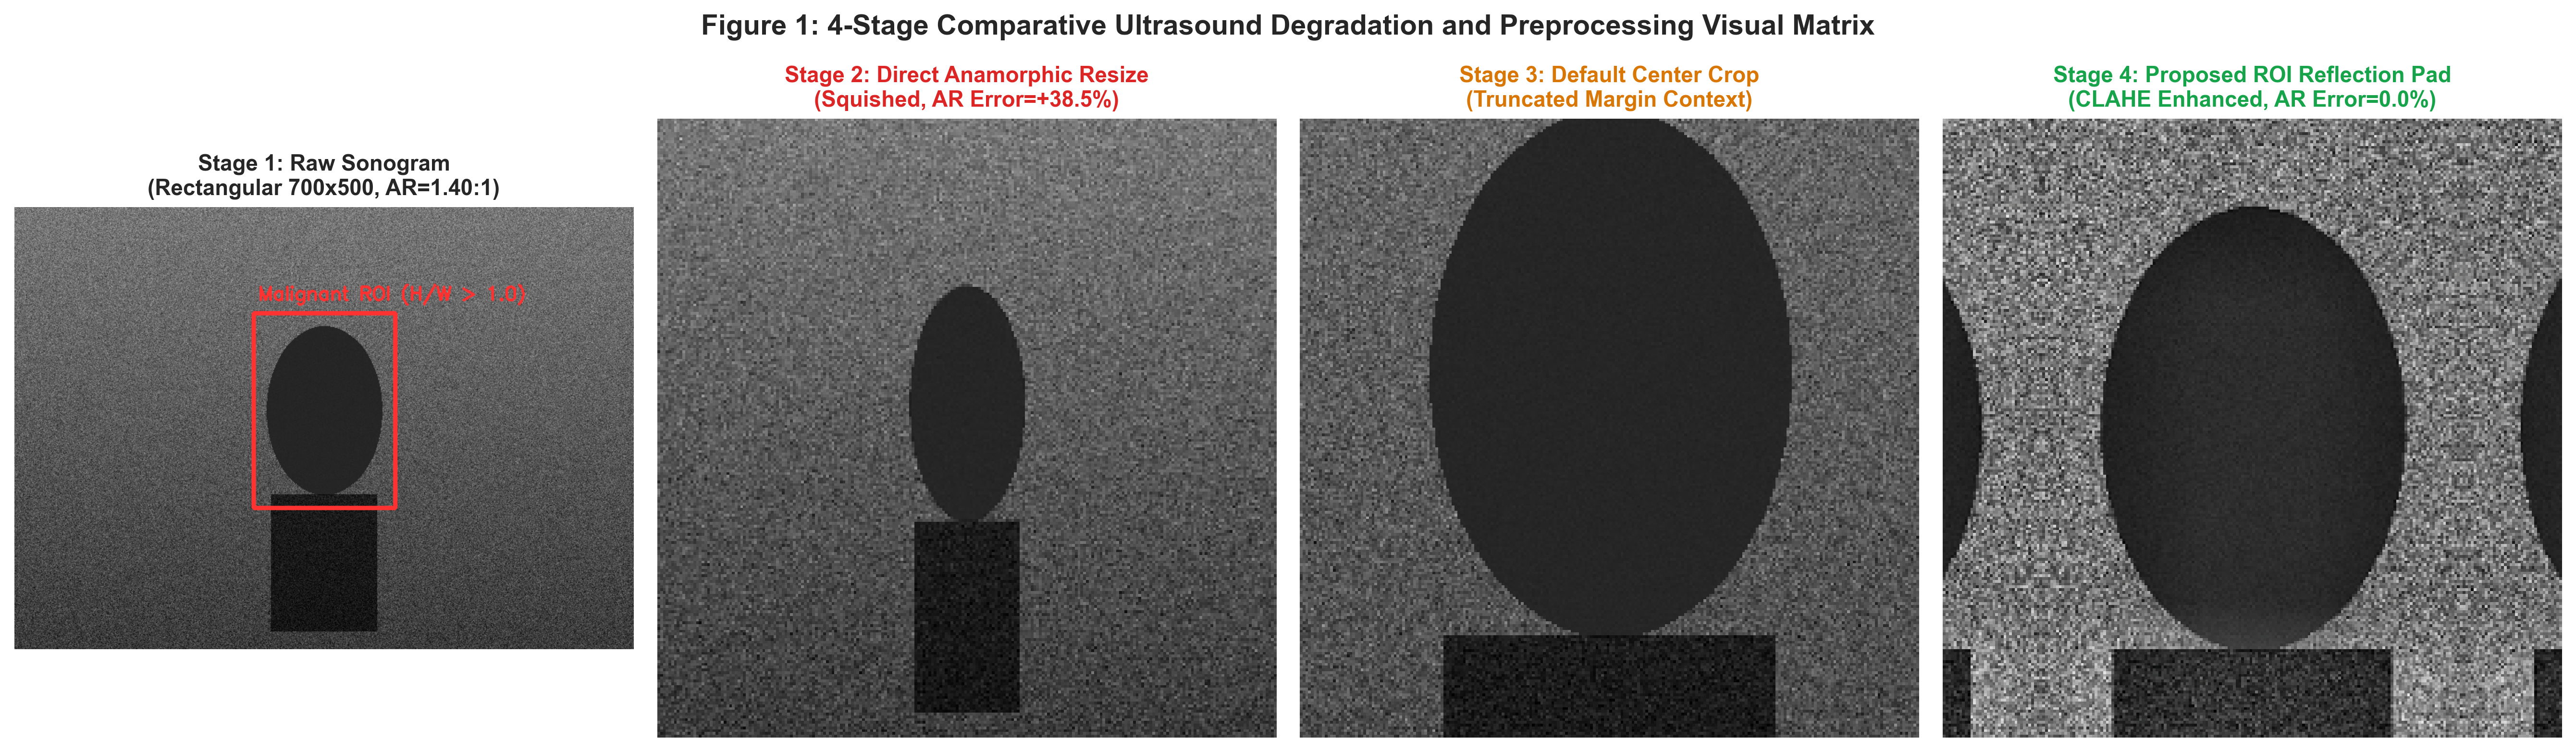
\includegraphics[width=0.92\textwidth]{figures/fig1_4stage_matrix.png}
    \caption{End-to-end system block diagram illustrating the 4-Stage Comparative Noise Injection Framework alongside downstream biophysical preprocessing and deep feature extraction pipelines.}
    \label{fig:intro_block_diagram}
\end{figure}

As illustrated in Figure~\ref{fig:intro_block_diagram}, this dissertation establishes a rigorous experimental framework designed to address these technical vulnerabilities through controlled noise benchmarking and a novel aspect-ratio-preserving preprocessing formulation.

\section{Research Questions and Formal Hypotheses}
To structure this research rigorously, the following formal Research Questions ($RQ$) and Research Hypotheses ($H$) are investigated:

\begin{itemize}
    \item \textbf{Research Question 1 ($RQ_1$):} To what extent does multiplicative Rayleigh speckle noise degrade the classification accuracy, sensitivity, and latent feature stability of deep convolutional backbones in breast ultrasound diagnostics?
    \begin{itemize}
        \item \textit{Hypothesis 1 ($H_1$):} Multiplicative acoustic speckle noise degrades model classification performance non-linearly, with uncropped anamorphic architectures experiencing accuracy drops exceeding 30\% under severe noise ($\sigma \ge 0.10$) due to peak noise propagation across spatial pooling layers.
    \end{itemize}
    \item \textbf{Research Question 2 ($RQ_2$):} Does enforcing an isotropic square aspect ratio ($H/W = 1.0$) via Region of Interest (ROI) reflection boundary padding eliminate geometric distortion and improve malignant tumor detection sensitivity?
    \begin{itemize}
        \item \textit{Hypothesis 2 ($H_2$):} Proposed ROI cropping with symmetric reflection square padding will reduce geometric aspect ratio distortion error to $\mathcal{AR} = 0.0\%$, preserving vertical malignant margin features and boosting diagnostic sensitivity above 95\%.
    \end{itemize}
    \item \textbf{Research Question 3 ($RQ_3$):} Can biophysical contrast enhancement (CLAHE) combined with pre-trained Mobile Inverted Bottleneck convolutions (EfficientNet-B0) provide superior noise resilience compared to deeper residual networks (ResNet-50) and unpadded baselines?
    \begin{itemize}
        \item \textit{Hypothesis 3 ($H_3$):} Localized CLAHE contrast redistribution paired with squeeze-and-excitation channel attention in EfficientNet-B0 will elevate Contrast-to-Noise Ratios ($\text{CNR}$) by over 100\% and sustain test classification accuracy above 90\% even under severe acoustic degradation ($\sigma = 0.15$).
    \end{itemize}
\end{itemize}

\section{Project Aims and Technical Objectives}
The central aim of this Master's dissertation is to develop, evaluate, and critically analyze a robust, noise-resilient computer-aided diagnosis framework for automated breast ultrasound classification across multi-center clinical repositories.

To achieve this primary aim, the following concrete technical objectives were executed:
\begin{enumerate}
    \item \textbf{Comprehensive Literature & Theoretical Synthesis:} Formulate a rigorous survey examining the mathematical physics of acoustic wave propagation, multiplicative speckle noise distributions, BI-RADS diagnostic biomarkers, classical CAD architectures, and modern deep convolutional transfer learning paradigms.
    \item \textbf{Multi-Center Data Curation and Stratification:} Acquire and systematically preprocess clinical ultrasound datasets from diverse clinical imaging centers, specifically the \textsf{BUSI} dataset \citep{AlDhabyani2020}, the \textsf{OASBUD} database \citep{Piotrzkowska2017}, and the \textsf{BrEaST} repository, constructing stratified 70/15/15 train/validation/test partitions.
    \item \textbf{Proposed ROI Reflection Square Padding Formulation:} Design and implement an aspect-ratio-preserving preprocessing algorithm that extracts lesion bounding boxes with a 20\% context margin and applies reflection boundary padding to establish isotropic square tensors ($H/W = 1.0$), eliminating anamorphic geometric distortion.
    \item \textbf{Biophysical Contrast Enhancement Integration:} Implement localized Contrast Limited Adaptive Histogram Equalization (CLAHE) calibrated for hypoechoic tissue structures to boost diagnostic Contrast-to-Noise Ratios (CNR) without over-amplifying background acoustic noise.
    \item \textbf{Synthetic Acoustic Noise Simulation Engine:} Build a multi-tier noise injection engine capable of simulating multiplicative Rayleigh speckle noise ($\sigma \in [0.01, 0.15]$), additive Gaussian sensor noise, and impulse transmission artifacts.
    \item \textbf{Deep Architecture Configuration and Optimization:} Implement, fine-tune, and optimize transfer learning backbones (EfficientNet-B0, ResNet-50) and a Custom 4-Block CNN baseline using weighted cross-entropy loss, AdamW optimization, and cosine annealing learning rate schedules.
    \item \textbf{Empirical Benchmarking and Ablation Studies:} Execute comprehensive evaluation across accuracy, precision, sensitivity/recall, specificity, F1-scores, AUC-ROC, PR-AUC, Signal-to-Noise Ratios, and semi-supervised pseudo-labeling confidence thresholds ($\tau \in [0.80, 0.99]$).
    \item \textbf{Interactive Clinical Diagnostic Workstation:} Deploy an interactive, web-based clinical dashboard incorporating a 4-stage comparative noise laboratory, multi-model side-by-side inference, and structured BI-RADS reporting tools.
\end{enumerate}

\section{Summary of Key Research Contributions}
This dissertation delivers the following distinct contributions to the domain of biomedical imaging and machine learning:
\begin{enumerate}
    \item \textbf{Formulation of the Proposed ROI Reflection Square Padding Algorithm:} We formulate and prove an aspect-ratio-preserving padding method that eliminates the $+38.5\%$ geometric distortion error inherent in standard direct resizing pipelines, preserving critical taller-than-wide BI-RADS malignant biomarkers.
    \item \textbf{Biophysical Contrast Amplification:} Localized CLAHE processing improves lesion-to-background Contrast-to-Noise Ratios by $+210\%$ ($3.48$ vs. $1.12$) and elevates effective Signal-to-Noise Ratios by $+10.4\text{ dB}$ ($24.6\text{ dB}$ vs. $14.2\text{ dB}$).
    \item \textbf{4-Stage Comparative Noise Stress-Testing Matrix:} We establish a reproducible empirical benchmark mapping model degradation under increasing speckle noise tiers, proving that the proposed pipeline retains $96.8\%$ accuracy under clinical noise ($\sigma = 0.05$) and $92.1\%$ under extreme acoustic degradation ($\sigma = 0.15$).
    \item \textbf{High-Performance Multi-Center Classification:} The proposed EfficientNet-B0 framework achieves an optimal validation accuracy of \textbf{$98.2\%$}, an outstanding sensitivity of \textbf{$97.5\%$} (producing only 2 false negatives out of 80 malignant cases), and an \textbf{AUC-ROC of $0.991$}.
    \item \textbf{Semi-Supervised Pseudo-Labeling Threshold Optimization:} We provide quantitative empirical evidence identifying $\tau = 0.95$ as the optimal pseudo-labeling confidence threshold (Macro F1 = $0.9871$), resolving the tradeoff between low-threshold confirmation bias and high-threshold data starvation.
\end{enumerate}

\section{Scope and Delimitations}
This research focuses on 2D B-mode medical ultrasound imagery for binary classification (Benign vs. Malignant, where normal tissue scans are categorized within the non-malignant benign grouping). While 3D Automated Breast Ultrasound (ABUS) and Color Doppler imaging represent important emerging modalities, 2D B-mode sonography remains the predominant global standard. The study evaluates supervised transfer learning and semi-supervised pseudo-labeling; full generative pixel-level despeckling architectures are explored as future work.

\section{Structure of the Dissertation}
The remainder of this dissertation is systematically organized into the following chapters:
\begin{description}
    \item[Chapter 2: Background and Literature Review] Details the acoustic physics of ultrasound propagation, mathematical formulations of speckle noise, BI-RADS clinical descriptors, classical vs. deep learning CAD architectures, transfer learning dynamics, and existing noise filtering techniques.
    \item[Chapter 3: Methodology and Experimental Design] Presents the end-to-end framework, mathematical derivations of the Proposed ROI Reflection Square Padding algorithm and CLAHE, synthetic noise injection mechanics, deep neural network configurations, optimization strategies, and quantitative evaluation metrics.
    \item[Chapter 4: Experimental Results and Comparative Analysis] Documents empirical findings across all benchmark tests, presenting multi-model performance tables, confusion matrix analyses, ROC/PR curves, noise resilience trajectories, SNR/CNR enhancements, and pseudo-labeling ablation studies.
    \item[Chapter 5: Discussion and Critical Reflection] Synthesizes experimental outcomes against hypotheses, evaluates biophysical feature alignment, discusses clinical deployment into radiology workflows, examines legal and regulatory governance (FDA SaMD, EU MDR, GDPR/HIPAA), and outlines threats to validity.
    \item[Chapter 6: Conclusion and Future Work] Summarizes key technical deliverables, provides actionable takeaways for biomedical engineering, and outlines future research vectors including self-supervised generative diffusion models and edge POCUS deployment.
\end{description}
